


\tikzset{every picture/.style={line width=0.75pt}} %set default line width to 0.75pt

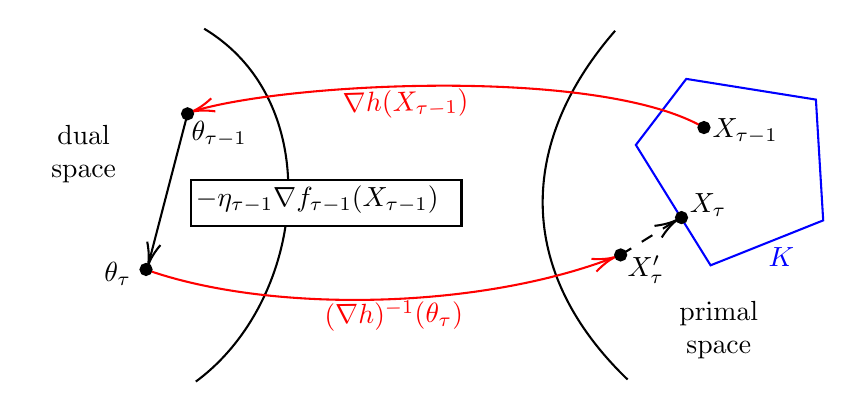
\begin{tikzpicture}[x=0.75pt,y=0.75pt,yscale=-1,xscale=1]
%uncomment if require: \path (0,308); %set diagram left start at 0, and has height of 308

%Curve Lines [id:da740927750098304]
\draw    (114.52,43.05) .. controls (174.52,79.05) and (163.52,174.05) .. (110.52,213.05) ;
%Curve Lines [id:da195036215046134]
\draw    (312.52,44.05) .. controls (265.52,98.05) and (264.52,160.05) .. (318.52,212.05) ;
%Shape: Boxed Polygon [id:dp43263390268315804]
\draw  [color=blue,draw opacity=1 ] (412.78,135.4) -- (358.52,157.05) -- (322.52,99.05) -- (346.81,67.23) -- (409.27,77.2) -- cycle ;
%Curve Lines [id:da4073635308662522]
\draw [color=red  ,draw opacity=1 ]   (110.58,82.42) .. controls (157.06,68.82) and (305.29,61.49) .. (355.33,90.67) ;
\draw [shift={(108.52,83.05)}, rotate = 342.35] [color=red  ,draw opacity=1 ][line width=0.75]    (10.93,-3.29) .. controls (6.95,-1.4) and (3.31,-0.3) .. (0,0) .. controls (3.31,0.3) and (6.95,1.4) .. (10.93,3.29)   ;
%Shape: Circle [id:dp9467983506453392]
\draw  [fill={rgb, 255:red, 0; green, 0; blue, 0 }  ,fill opacity=1 ] (103.86,84.05) .. controls (103.86,82.57) and (105.05,81.38) .. (106.52,81.38) .. controls (108,81.38) and (109.19,82.57) .. (109.19,84.05) .. controls (109.19,85.52) and (108,86.71) .. (106.52,86.71) .. controls (105.05,86.71) and (103.86,85.52) .. (103.86,84.05) -- cycle ;
%Shape: Circle [id:dp9056670319943894]
\draw  [fill={rgb, 255:red, 0; green, 0; blue, 0 }  ,fill opacity=1 ] (352.67,90.67) .. controls (352.67,89.19) and (353.86,88) .. (355.33,88) .. controls (356.81,88) and (358,89.19) .. (358,90.67) .. controls (358,92.14) and (356.81,93.33) .. (355.33,93.33) .. controls (353.86,93.33) and (352.67,92.14) .. (352.67,90.67) -- cycle ;
%Straight Lines [id:da7607534724135314]
\draw    (106.52,84.05) -- (88.03,155.11) ;
\draw [shift={(87.52,157.05)}, rotate = 284.59000000000003] [color={rgb, 255:red, 0; green, 0; blue, 0 }  ][line width=0.75]    (10.93,-3.29) .. controls (6.95,-1.4) and (3.31,-0.3) .. (0,0) .. controls (3.31,0.3) and (6.95,1.4) .. (10.93,3.29)   ;
%Curve Lines [id:da4928498947155546]
\draw [color=red  ,draw opacity=1 ]   (89.19,160.05) .. controls (148.23,179.95) and (246.06,178.44) .. (311.54,153.43) ;
\draw [shift={(312.52,153.05)}, rotate = 518.81] [color=red  ,draw opacity=1 ][line width=0.75]    (10.93,-3.29) .. controls (6.95,-1.4) and (3.31,-0.3) .. (0,0) .. controls (3.31,0.3) and (6.95,1.4) .. (10.93,3.29)   ;
%Shape: Circle [id:dp6963694929251834]
\draw  [fill={rgb, 255:red, 0; green, 0; blue, 0 }  ,fill opacity=1 ] (83.86,159.05) .. controls (83.86,157.57) and (85.05,156.38) .. (86.52,156.38) .. controls (88,156.38) and (89.19,157.57) .. (89.19,159.05) .. controls (89.19,160.52) and (88,161.71) .. (86.52,161.71) .. controls (85.05,161.71) and (83.86,160.52) .. (83.86,159.05) -- cycle ;
%Shape: Circle [id:dp9345908069488471]
\draw  [fill={rgb, 255:red, 0; green, 0; blue, 0 }  ,fill opacity=1 ] (312.52,152.05) .. controls (312.52,150.57) and (313.72,149.38) .. (315.19,149.38) .. controls (316.66,149.38) and (317.86,150.57) .. (317.86,152.05) .. controls (317.86,153.52) and (316.66,154.71) .. (315.19,154.71) .. controls (313.72,154.71) and (312.52,153.52) .. (312.52,152.05) -- cycle ;
%Shape: Circle [id:dp26656479634987873]
\draw  [fill={rgb, 255:red, 0; green, 0; blue, 0 }  ,fill opacity=1 ] (341.86,134.05) .. controls (341.86,132.57) and (343.05,131.38) .. (344.52,131.38) .. controls (346,131.38) and (347.19,132.57) .. (347.19,134.05) .. controls (347.19,135.52) and (346,136.71) .. (344.52,136.71) .. controls (343.05,136.71) and (341.86,135.52) .. (341.86,134.05) -- cycle ;
%Straight Lines [id:da12825213670576918]
\draw  [dash pattern={on 4.5pt off 4.5pt}]  (315.19,152.05) -- (340.83,136.1) ;
\draw [shift={(342.52,135.05)}, rotate = 508.12] [color={rgb, 255:red, 0; green, 0; blue, 0 }  ][line width=0.75]    (10.93,-3.29) .. controls (6.95,-1.4) and (3.31,-0.3) .. (0,0) .. controls (3.31,0.3) and (6.95,1.4) .. (10.93,3.29)   ;

% Text Node
\draw (385,147) node [anchor=north west][inner sep=0.75pt]  [color=blue  ,opacity=1 ]  {$K$};
% Text Node
\draw (179.66,72) node [anchor=north west][inner sep=0.75pt]  [color=red  ,opacity=1 ,rotate=-358.33]  {$\nabla h( X_{\tau -1})$};
% Text Node
\draw (170.87,173) node [anchor=north west][inner sep=0.75pt]  [color=red  ,opacity=1 ,rotate=-359.31]  {$( \nabla h)^{-1}( \theta _{\tau })$};
% Text Node
\draw (358,85) node [anchor=north west][inner sep=0.75pt]    {$X_{\tau -1}$};
% Text Node
\draw (347,121) node [anchor=north west][inner sep=0.75pt]    {$X_{\tau }$};
% Text Node
\draw (317,151) node [anchor=north west][inner sep=0.75pt]    {$X'_{\tau }$};
% Text Node
\draw (65,154) node [anchor=north west][inner sep=0.75pt]    {$\theta _{\tau }$};
% Text Node
\draw (107,86) node [anchor=north west][inner sep=0.75pt]    {$\theta _{\tau -1}$};
% Text Node
\draw  [fill={rgb, 255:red, 255; green, 255; blue, 255 }  ,fill opacity=1 ]  (108,116.05) -- (238.52,116.05) -- (238.52,138) -- (108,138) -- cycle  ;
\draw (109,117.05) node [anchor=north west][inner sep=0.75pt]    {$-\eta _{\tau -1} \nabla f_{\tau -1}( X_{\tau -1})$};
% Text Node
\draw (30,88) node [anchor=north west][inner sep=0.75pt][align=left] {\begin{minipage}[lt]{37.43pt}\setlength\topsep{0pt}
\begin{center}
dual\\space
\end{center}

\end{minipage}};
% Text Node
\draw (336,173) node [anchor=north west][inner sep=0.75pt][align=left] {\begin{minipage}[lt]{37.43pt}\setlength\topsep{0pt}
\begin{center}
primal\\space
\end{center}

\end{minipage}};


\end{tikzpicture}
